%%%%%%%%%%%%%%%%%%%%%%%%%%%%%%%%%%%%%%%%%%%%%%%%%%%%%%%%%%%%%%%%%%%%%%%%%%%%%%%%%%%%%%%%%
%%%%%%%%%%%%%%%%%%%%%%%%%%%%%%%%%%%%%%%%%%%%%%%%%%%%%%%%%%%%%%%%%%%%%%%%%%%%%%%%%%%%%%%%%
%%%%%%%%%%%%%%%%%%%%%%%%%%%%%%%%%%%%%%%%%%%%%%%%%%%%%%%%%%%%%%%%%%%%%%%%%%%%%%%%%%%%%%%%%

%\td{https://en.wikipedia.org/wiki/Thesis}
%\ds{what is it? What is it used for? How does it work? What different kinds are there? }
%\ds{what? how? why?}
This chapter can be broken down into three sections. 
The first section tries to shine light on the evolution of PV and give some background information on \gls{cigs} absorber.
The next section concerns the description of materials and scientific methods used during the experinental part of this work. 
The third and last part focuses on the algorithmic, statistical and analytical methods used to optimize and predict material properties. 

%%%%%%%%%%%%%%%%%%%%%%%%%%%%%%%%%%%%%%%%%%%%%%%%%%%%%%%%%%%%%%%%%%%%%%%%%%%%%%%%%%%%%%%%%
%%%%%%%%%%%%%%%%%%%%%%%%%%%%%%%%%%%%%%%%%%%%%%%%%%%%%%%%%%%%%%%%%%%%%%%%%%%%%%%%%%%%%%%%%%%%%
%%%%%%%%%%%%%%%%%%%%%%%%%%%%%%%%%%%%%%%%%%%%%%%%%%%%%%%%%%%%%%%%%%%%%%%%%%%%%%%%%%%%%%%%%
\section{Photovoltaics}
%\subsection{Problems of current energy supply}
The world wide energy consumption has more than doubled between 1970 and 2015\cite{BP2017} 
and according to recent studies both fossil\cite{BGR2017} and uranium sources\cite{Uran2006} 
will be exhausted within the next 100 years. 
Even though this time period is not exact and highly dependent on detection methods of resources, 
the situation demands the fast 
development of sustainable energy sources. 
% this number is rather small and brings us in \textit{zugzwang} to develop sustainable energy sources. 
One viable option is \gls{pv}.

%%%%%%%%%%%%%%%%%%%%%%%%%%%%%%%%%%%%%%%%%%%%%%%%%%%%%%%%%%%%%%%%%%%%%%%%%%%%%%%%%%%%%%%%%%%%%
\subsection{History of Photovoltaics}
The photoelectric effect was first described in 1839 by french scientist Alexandre 
Edmond \linebreak[4] 
Becquerel\cite{becquerel1839memoire}. %, the father of Henri Becquerel (the person after whom the unit is named).
Another relevant piece in the \gls{pv} jigsaw was brought to light
%discovered
with the discovery of photo conductivity of selenium
by British engineer Willouhgby Smith\cite{Smith1873Selenium}.
In 1876 William Adams and Richard Day\cite{Adams1876Selenium} showed that 
the energy of light can be directly converted into electrical energy by a bar of 
selenium with attached platinum electrodes.
And finally, in 1905 Einstein described the physical background of the photoelectric 
effect with his light quantum theory\cite{einstein1905erzeugung}.
%\todo{https://doi.org/10.1063/1.1716492}
In the late 1950s the first solar cells (with power conversion efficiencies around 10 percent\cite{prince1958}) were used in niche applications such as space exploration.  
In 1958 the US American Vanguard I\cite{vanguard2004} and the soviet Sputnik III\cite{sputnik1959} were the first satellites with solar cells.
These "solar batteries" - as they were called then - allowed the transmission system of Vanguard I to be operating for over a year after the chemical battery powered system stopped transmitting after 20 days\cite{vanguard2004}. 
%
Eventually, the interest in photovoltaic and other alternative energy sources 
rose - fuelled by the oil crisis in 1973 - 
and the development of photovoltaic devices for the consumer market was boosted. 
This development lead to a drop in 
average price for \gls{pv} module from \$ 100 per watt in 1975 
%to \$ 4 per watt in 2007\cite{pagliaro2008flexible}. 
to under \$ 1 per watt in 2022\cite{irena2023renewable}.

%%%%%%%%%%%%%%%%%%%%%%%%%%%%%%%%%%%%%%%%%%%%%%%%%%%%%%%%%%%%%%%%%%%%%%%%%%%%%%%%%%%%%%%%%%%%%
\subsection{Photovoltaics Basics}
The process of conversion of photons into electric energy can be broken down into two essential steps: 
the generation of an electron-hole pair through photon absorption, the electron-hole separation by the built in electric field at the p-n junction and finally collection of the electrons and holes at the opposite terminals of the device\cite{markvart2013principles}.
This means that \gls{pv} cells are basically diodes, which have a low resistance in one direction and a high resistance in the other direction. 
%This is often achieved through a p-n junction.
The n-type side of the p-n junction has excess electrons and p-type side has excess electron holes. 
If the n- and p-type are of the same basis material, they are called homojunctions (e.g.\ silicon); if not, heterojunctions (e.g.\ \ch{CdS}/\gls{cigs} and \ch{CdS/CdTe})\cite{breitenstein2013understanding}.
%
The first marketable \gls{pv} were crystalline silicon photovoltaic modules which still 
have the biggest market share in the \gls{pv} segment (including polycrystalline and monocrystalline silicon).
In 2022 over 88\% of all sold \gls{pv} where made of silicon (including amorphous silicon)\cite{breitenstein2013understanding}.
%
A comprehensive overview on different \gls{pv} technologies can be found in \cite{markvart2013principles}.


%%%%%%%%%%%%%%%%%%%%%%%%%%%%%%%%%%%%%%%%%%%%%%%%%%%%%%%%%%%%%%%%%%%%%%%%%%%%%%%%%%%%%%%%%%%%%
\subsection{Copper Indium Gallium Selenide Solar Cell}
%\subsection{Copper Indium Gallium Selenide} 
\gls{cigs} (\ch{CuIn_{x}Ga_{1-x}Se2}) is of the chalcopyrite (\ch{CuFeS2}) group (tetragonal crystal system). 
%It was 
\ch{CuInSe2} and \ch{CuGaSe2} were first synthesised in 1953 by Harry Hahn et al.\cite{hahn1953untersuchungen}.
The potential use of \ch{CuInSe2} as \gls{pv} material in combination with \ch{CdS} was first mentioned in 1974\cite{wagner1974cuinse2}.
%Already in 1975 efficiencies of cells of over 10\% were achieved.\cite{kazmerski1976thin}
Cells with efficiencies of over 10\% were achieved already by 1975\cite{kazmerski1976thin}.
Today, 
\gls{cigs} (multiple \gls{pv} cells in series) 
reach efficiencies of up to 19\%,
monocrystalline silicon \gls{pv} modules reach efficiencies of 24\%
and polycrystalline silicon \gls{pv} modules 20\%\cite{green2023solar}.

Just like CdTe, GaAs and amorphous silicon solar cells, CIGS has much higher absorption coefficients of UV, visible and IR light than crystalline silicon (see table \ref{tab:cigs:alpha}). 
This is due to a direct band gap rather than an indirect band gap (like crystalline silicon). 
These thin film \gls{pv}s not only use less material, but also can be used in flexible applications. 

\begin{table}[tbh]
	\small
    \center
	\resizebox{\textwidth}{!}{
		\begin{tabular}{cccccc}
			\hline
			\hline
			Material&   Type&    Band Gap [\ev{}]&    $\lambda$ [\nm{}]&    Abs. coef. $\alpha$ [\pcm{}]    &Penetration Depth [\um{}]\\
			\hline
			c-Si&   indirect&   1.12&   600&    \num{4000}&    2.5\\
			c-Si&   indirect&   1.12&   1000&    \num{64}&    150\\
			c-Si&   indirect&   1.12&   1100&    \num{3.5}&    290\\
			a-Si&   direct&      1.7&    600&    \num{40000}&  0.25\\
			CdTe&   direct&      1.45&    600&    \num{37000}&  0.3\\
			GaAs&   direct&      1.42&    600&    \num{40000}&  0.2\\
			\hline
			\hline
		\end{tabular}
	}
    \caption{Photonic properties of several established \gls{pv} materials (data from \cite{mertens2020photovoltaik})}
	\label{tab:cigs:alpha}
%
	\vspace{1cm}
    \begin{tabular}{cccc}
        \hline\hline
		Empirical Formula&    Name&   Band Gap [\si{eV}{}]&    Abbreviation\\
        \hline
		\ch{CuInSe2}&       copper indium di selenide&  1.04&  CISe\\
		\ch{CuInS2}&        copper indium di sulfide&  1.5&  CIS\\
		\ch{CuGaSe2}&       copper gallium di selenide&  1.7&  CIGSe\\
		\ch{CuGaS2}&        copper gallium di sulfide&  1.55&  CIGS\\
        \hline\hline
    \end{tabular}
    \caption{Band gaps of different chalcopyrites (data from \cite{mertens2020photovoltaik})}
	\label{tab:cigs}
\end{table}

\begin{figure}[tbh]
	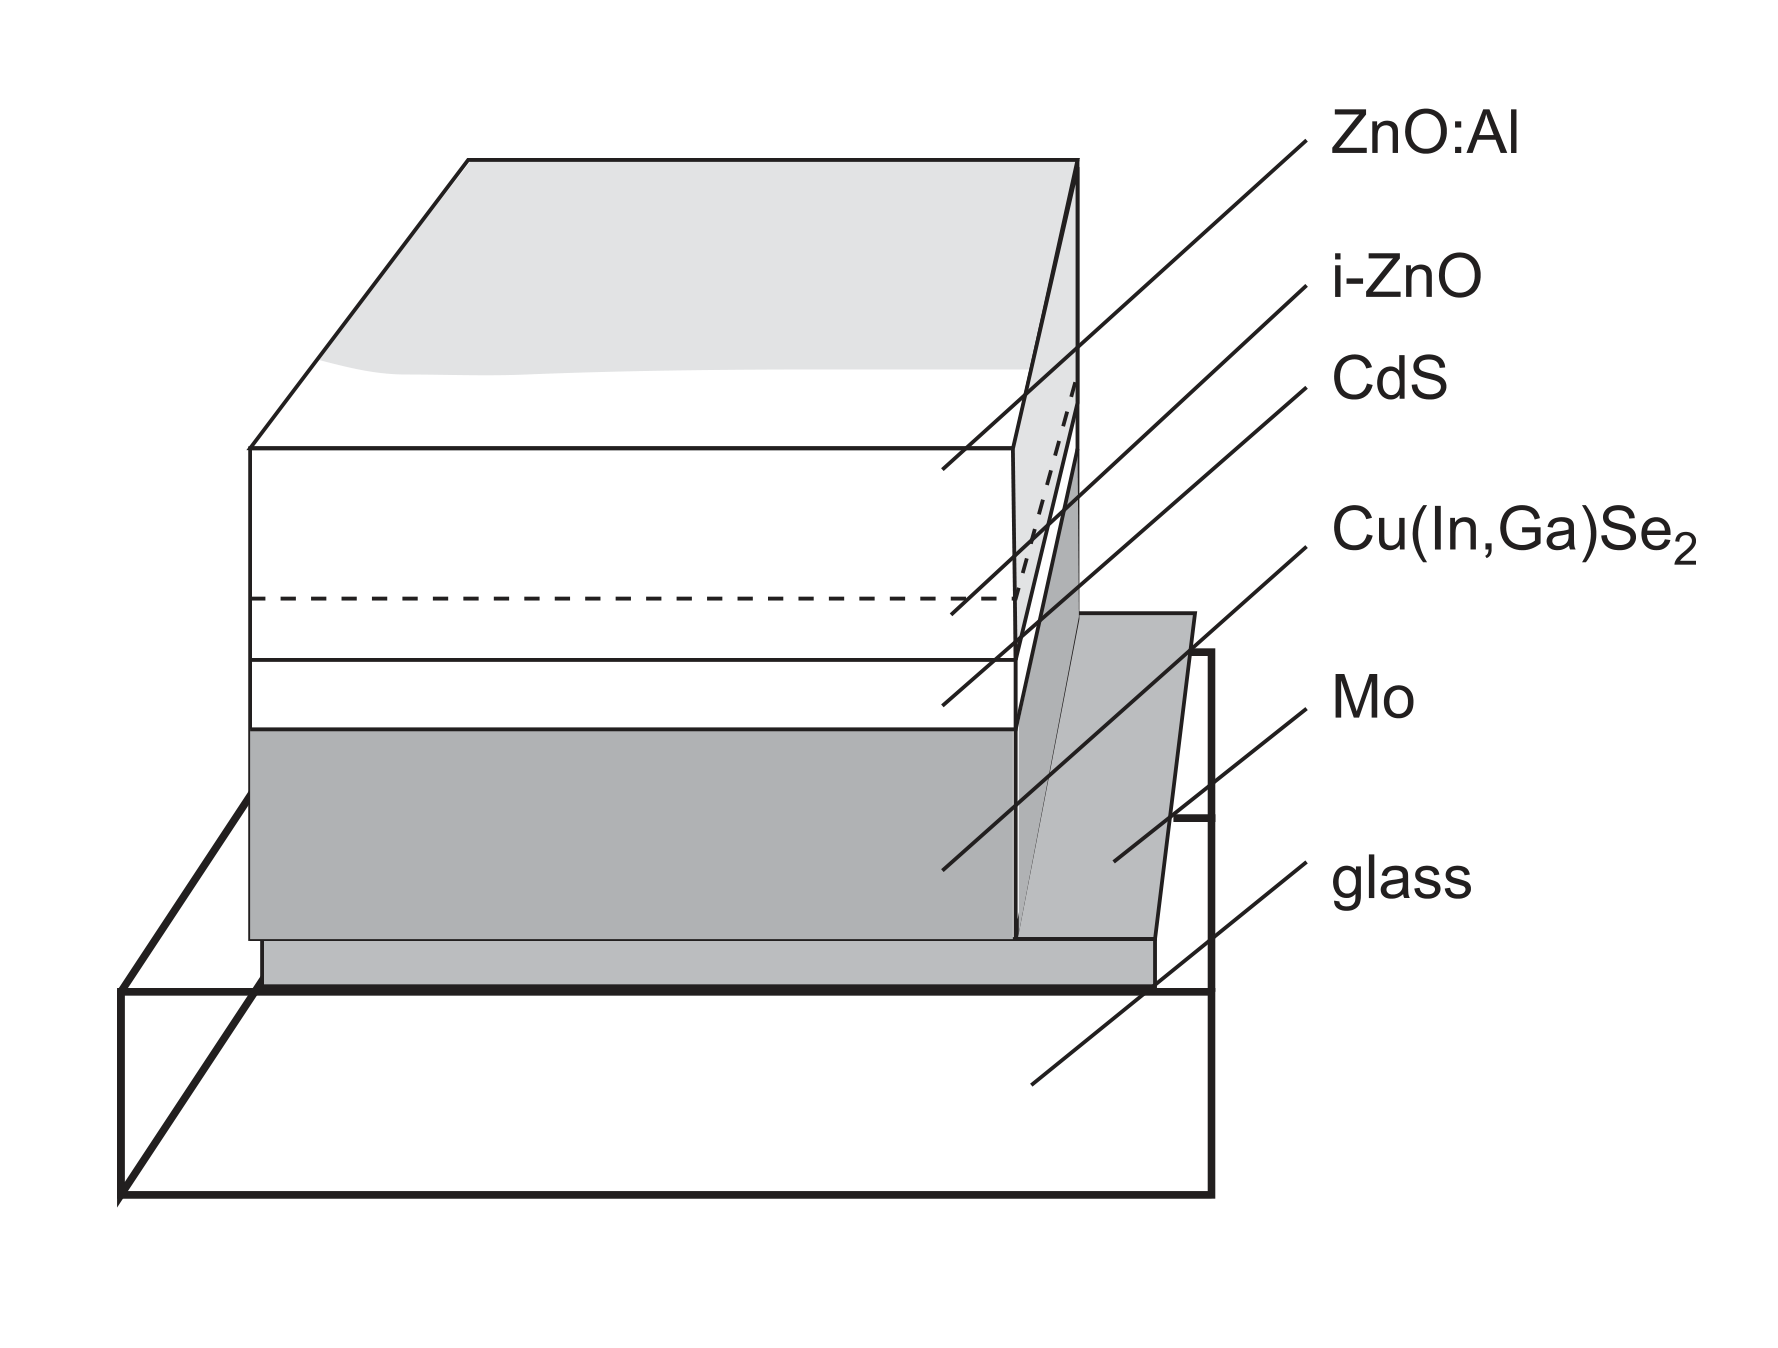
\includegraphics[width=\textwidth]{./Pics/cigs.png}
    \caption{Schematic layer sequence of a standard \ch{ZnO}/\ch{CdS}/\ch{Cu(In,Ga)Se2} thin-film solar cell\cite{rau2013cigs}.}
	\label{fig:cigs}
\end{figure}

The band gap of CIGS can be varied between \ev{1} and \ev{1.7} by varying the indium-gallium and sulfur-selenium ratios.
This is a result of the large difference of band gaps of \ch{CuInSe2} and \ch{CuGaSe2} (see table \ref{tab:cigs}). 
%%
%%%%%%%%%%%%%%%%%%%%%%%%%%%%%%%%%%%%%%%%%%%%%%%%%%%%%%%%%%%%%%%%%%%%%%%%%%%%%%%%%%%%%%%%%%%%%
In figure \ref{fig:cigs} the schematic layer sequence of a standard \gls{cigs} thin film cell is shown. 
Typically, a \um{1} thick molybdenum layer is deposited on soda lime glass. 
The sodium in the glass diffuses through the molybdenum layer and increases efficiency and reliability by directing the growth of \gls{cigs} in the 112 direction\cite{hedstrom1993cigs}.
A \gls{cigs} layer of 1-\um{2} thickness is applied on top via co-evaporation from elemental sources\cite{hedstrom1993cigs}.
The p-type doping of \gls{cigs} is achieved by adding more than stoichiometric copper to the mix. 
The heterojunction is then completed by deposition of \ch{CdS} n-type layer (typically \nm{50} thick).
\ch{CdS} was earlier used as front contact, but now only acts as n-type wide-gap window and buffer. 
After the \ch{CdS} layer 
A window layer of intrinsic \ch{ZnO} is deposited after the \ch{CdS}, followed by a highly conductive aluminium doped layer. 
\ch{ZnO} has a band gap of \ev{3.2} and is therefore transparent for visible light. 
The \ch{ZnO} window layer (usually of thickness 50-\nm{70} is highly conductive (especially the aluminium doped layer) and acts as front contact. 

%
Instead of glass as substrate, steel and polymers (e.g.\ polyimide\cite{feurer2017cigs}) can be used to create flexible \gls{cigs} modules. 
They both come with their own inconveniences. 
Polymers generally have low thermal stability compared with ceramics and metals which restrict the fabrication temperature of \gls{cigs}.
Steel, on the other hand, is temperature resistant enough, but is an electric conductor, which is problematic for the serial interconnection of cells into modules. 
Thus, an insulating layer has to be deposited on the steel substrate. 
%The conductance of steel can be masked by a insulator layer (e.g.\ \ch{ZrO2}, \ch{Al2O3}).

\pagebreak[4]
%%%%%%%%%%%%%%%%%%%%%%%%%%%%%%%%%%%%%%%%%%%%%%%%%%%%%%%%%%%%%%%%%%%%%%%%%%%%%%%%%%%%%%%%%%%%%
%%%%%%%%%%%%%%%%%%%%%%%%%%%%%%%%%%%%%%%%%%%%%%%%%%%%%%%%%%%%%%%%%%%%%%%%%%%%%%%%%%%%%%%%%%%%%
%%%%%%%%%%%%%%%%%%%%%%%%%%%%%%%%%%%%%%%%%%%%%%%%%%%%%%%%%%%%%%%%%%%%%%%%%%%%%%%%%%%%%%%%%%%%%

%\section{Materials and Their Analysis}
\section{Sample preparation}
%\todo{COATING OF THE SUBSTRATE or sample preparation}
%%%%%%%%%%%%%%%%%%%%%%%%%%%%%%%%%%%%%%%%%%%%%%%%%%%%%%%%%%%%%%%%%%%%%%%%%%%%%%%%%%%%%%%%%
\subsection{Properties of Zirconium oxide}
Zirconium oxide \gls{zro} is a ceramic with a band gap of 5-7 eV\cite{Anwar2017} and relative permittivity of circa 20 at room temperature\cite{kukli2001dielectric}. 
This makes it attractive as an insulator for semiconductor and \gls{pv} industry. 
It is monoclinic below 1050 °C, tetragonal between 1170 °C and 2370 °C, and cubic above 2370 °C\cite{Nielsen2005}.
The cubic phase can be stabilized down to room temperature by the addition of magnesia (\ch{MgO}), calcia (\ch{CaO}) or yttria (\ch{Y2O3}). 
This prevents mechanical failing due to shrinkage 
when cooling and undergoing phase transition\cite{Nielsen2005}.
\ch{ZrO2} is very resistant to acids (except \ch{HF} and hot \gls{h2so4}) and bases\cite{Nielsen2005}.
%Hydrous Zirconium Oxide (\ch{Zr(OH)8 * 16 H2O}) gel can be produced by neutral hydrolysis of sodium zirconate (\ch{NaZrO3})\cite{Nielsen2005}.
%"Zirconium alkoxides hydrolyze quite easily, [providing] a route to high purity, high-surface-area zirconium oxide"\cite{Nielsen2005}.

%%%%%%%%%%%%%%%%%%%%%%%%%%%%%%%%%%%%%%%%%%%%%%%%%%%%%%%%%%%%%%%%%%%%%%%%%%%%%%%%%%%%%%%%%%%
%\subsection{Sol-Gel and Doctor Blading}
\subsection{Tape Casting}
%\td{what is it? What is it used for? How does it work? What different kinds are there? }One of the advantages of sol-gel process is that it can be used in roll-to-roll procedures.
%
Tape casting (also known as tape casting) is widely used in the textile, paper, photographic film, printing and ceramic industries.
The roll-to-roll compatible process gives rise to highly uniform films over large areas\cite{yang2010large}.
A blade is moved over a substrate spreading a slurry at a fixed distance with a fixed speed.
In roll-to-roll processes the substrate moves instead of the blade. 

%%%%%%%%%%%%%%%%%%%%%%%%%%%%%%%%%%%%%%%%%%%%%%%%%%%%%%%%%%%%%%%%%%%%%%%%%%%%%%%%%%%%%%%%%%%
\subsection{Contact Deposition by Sputtering}
%SPUTTERING FREEWRITING: 
% what is sputtering?
Sputtering describes the process of highly energetic ions bombarding a surface and atoms being ejected from the surface as a consequence.
% what can it be used for? 
%It can be used for high precision etching (semiconductors and nanomaterial) or to deposit thin films. 
%
Use cases vary from thin films depositions for \gls{pv}, 
for electrical circuits or for storage media such as CDs and DVDs 
over sputter cleaning and etching to analysis.
Advantages of sputter-deposited thin films include good adhesion to the substrate 
and good step coverage\cite{Swann1988}.
% how does it work? 
%A plasma is created and the ions are accelerated to the surface. 
The ions, which are accelerated to the surface, mostly originate from a plasma.
The ion bombardment leads to a transfer of momentum from the ions to the surface atoms which in turn leads to a collision cascade. 
The cascade can reach the surface again. 
If the energy of an atom is larger than the binding energy, the atom is ejected. 
%If a surface particle obtains momentum pointing away from the bulk and its kinetic energy is higher than the binding energy, the particle is sputtered. 
This neutral ejected particle travels -- unaffected by the electrical field nearly perpendicular to the surface -- towards the substrate and condenses with other particles to form a layer.
The pressure in the chamber should be small, such that the sputtered particle has a long mean free path, but on the other hand 
a minimum pressure is needed to sustain the plasma.
Usual pressures are around \SI{1}{\Pa} (\num{e-2}\SI{}{\milli\bar}) or lower\cite{Swann1988}.
% what is used? 
Nobel gases (e.g.\ argon) in plasma phase are mainly used for bombardment because of their inert properties. 
Oxygen or nitrogen can be added to the plasma to deposit oxides or nitrides, respectively.
%Reactive gases can be added (e.g.\ \ch{O2} or \ch{N2}).
In order to use sputtering for depositing a target material on top of a substrate material, 
the target and the substrate are positioned parallel and in between the gas is transitioned into plasma and the ions are accelerated in the direction of the target (by a high electrostatic potential). 

\todo{what were the used settings: leybold etc.}
%Prior to \gls{iv} measurements the samples were sputtered with aluminium through a mask to produce a multitude of equidistant contacts with a Leybold UNIVEX450C Sputter System.
%Directional current sputtering was used with argon as inert gas at \SI{0.005}{\milli\bar} and with a power of \SI{40}{\watt} for \SI{700}{\second}.

%what is sputtering? \\
% Sputtering is the processes of highly energetic ions hitting a surface and atoms or molecules being expelled. 
%This is called a \gls{pvd} technique in contrast to chemical vapor deposition. 
%\Gls{pvd} can be divided into activation by thermal energy and activation by energetic particle bombardment. 
%Sputtering is of the latter kind, which is advantageous if substrates can not withstand high temperatures.
%\td{what can it be used for?}\\
%Sputtering evolved from being a curious experiment in the middle of the 20th century to 
%having various applications in research and engineering.

\begin{figure}[tbh]
    \centering
    \begin{subfigure}[t]{.3\textwidth}
        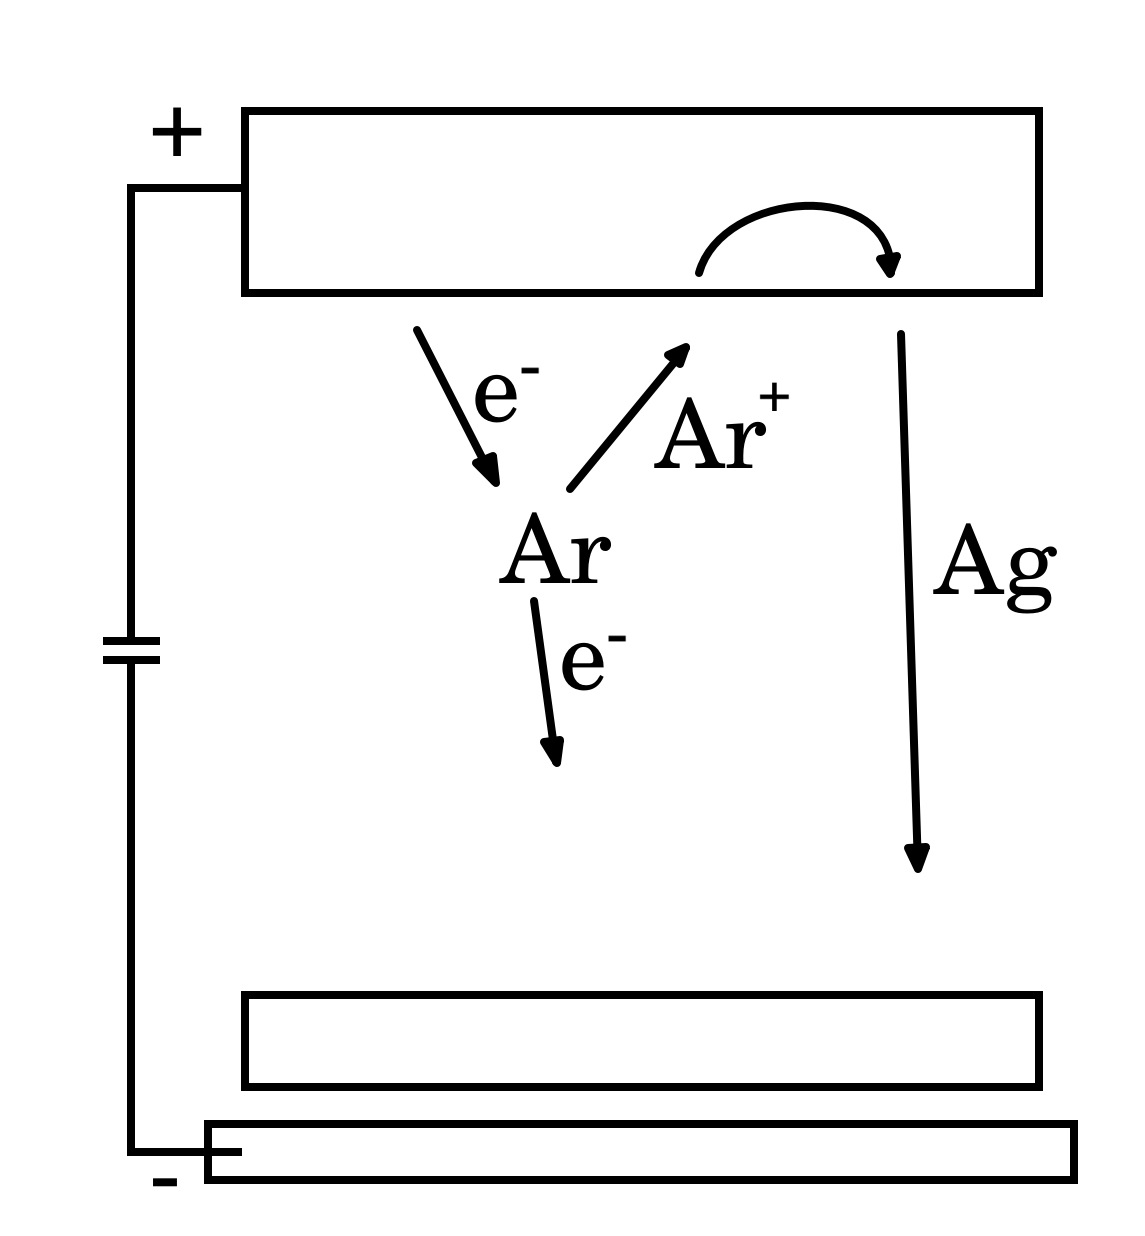
\includegraphics[width=\textwidth]{./Pics/sputter1.png}
        \caption{}
        \label{fig:sputter0}
    \end{subfigure}
    \hspace{1cm}
    \begin{subfigure}[t]{.3\textwidth}
        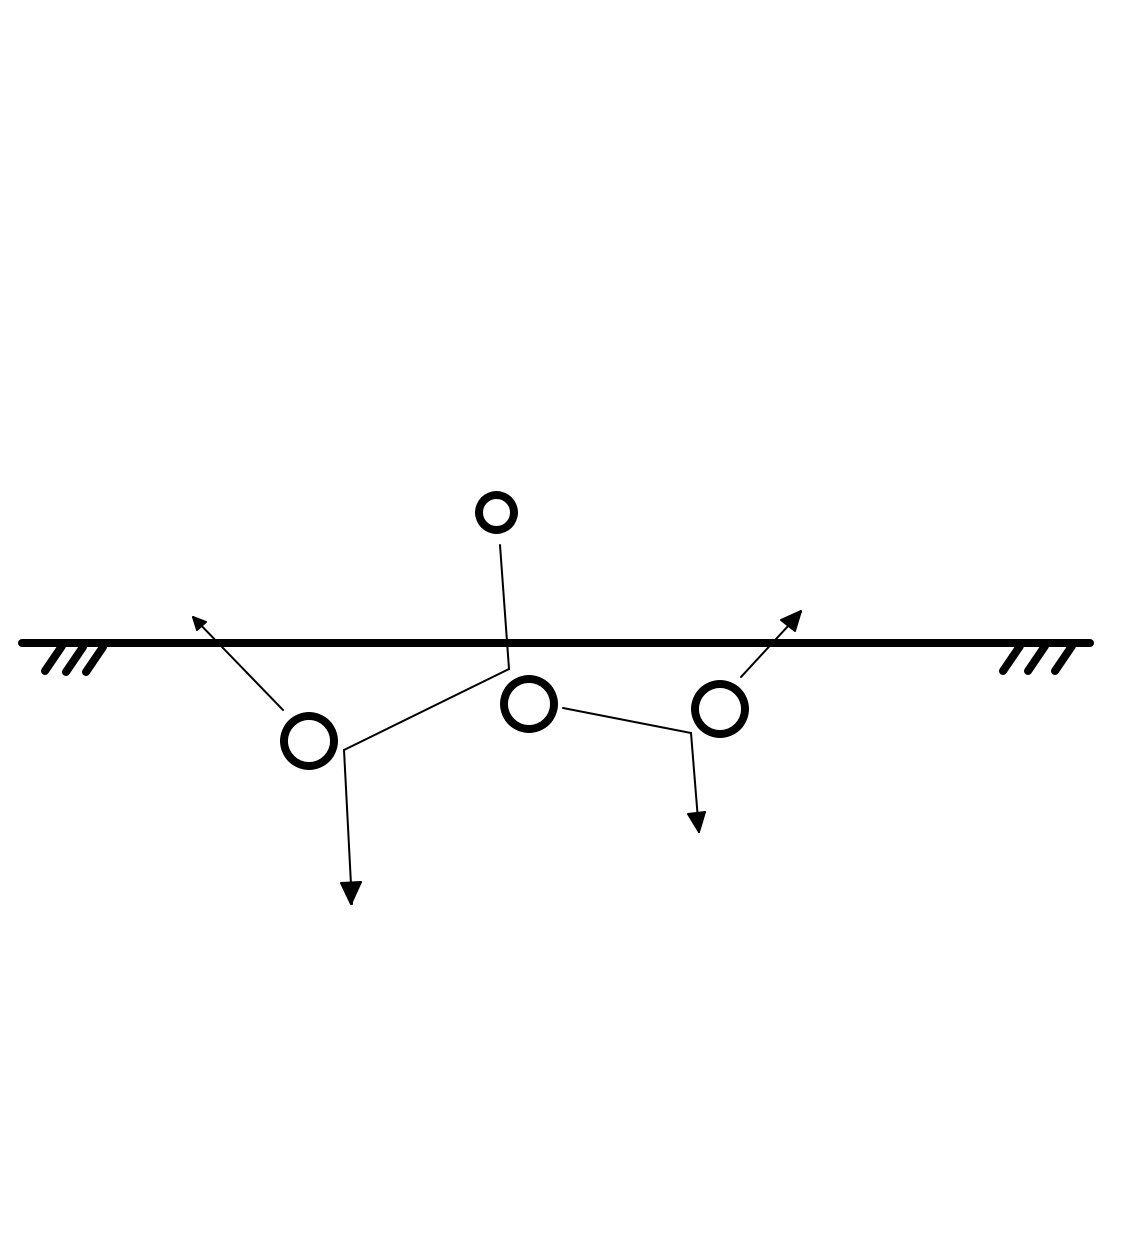
\includegraphics[width=\textwidth]{./Pics/sputter2.png}
        \caption{}
        \label{fig:sputter1}
    \end{subfigure}
%    \caption{Propagation of energy in a dense cascade. Left graph: "Primary" shockwave. Right graph: "Thermal" pulse or "secondary" shockwave. Figure taken from Sigmund 1987\cite{sigmund1969}}
    \caption{Schematic representation of the creation of sputter particles during sputter deposition. 
    (a)~creation of ions in the chamber: 
        the top rectangle depicts the source/cathode/target, 
        the bottom rectangle the anode/substrate holder and 
        the middle rectangle the substrate to be sputtered. 
    (b) example series of collision processes leading to sputtering of atoms: 
        horizontal line represents the target surface, 
        the small circle a high energetic ion and 
        the large circles target particles. 
    }
	\label{fig:sputter}
\end{figure}

\iffalse
%\td{how does it work?}\\
A high voltage is applied to 
two parallel electrodes with low pressure gas in between. 
The target acts as as feedstock anode and the substrate (holder) as cathode (see figure \ref{fig:sputter0}).
%the target which acts as a cathode with the substrate as anode in a parallel geometry (see \td{fig}).
The anode, then, emits electrons which collide with gas particles (mostly argon because of its inert nature and potential to transfer more kinetic than lighter noble gases). 
Some gas particles may get ionized by the collision and the gas cations are accelerated to the anode. 
If a cation has enough energy, it will bump off one or more atoms or molecules from the surface. 
This happens by a cascade of momentum transfers, which can reach the surface again (see figure \ref{fig:sputter1}). 
\fi


\iffalse
A magnetron can be placed behind the cathode (target) in order to trap the plasma close to the source. 
This lowers the pressure needed to sustain the plasma. 
Furthermore, magnetrons prevent high energy electrons from reaching the substrate and 
undoing the deposited layer.
This also increases the probability of an electron 
colliding with an argon atom and ionizing it, increasing the yield.
%
When oxygen or nitrogen are added to the gas this is called reactive sputtering.
Sputtered atoms will react with the gas and result in oxide or nitride layers, respectively.
The stoichiometry of the resulting layer can be regulated by gas ratios, but too much reactive gas can lead to target poisoning;
meaning that the target is being passivated by an insulating layers which can lead to defects in the growing film\cite{Kelly2000}. 
%
The limitation of only being able to use conducting materials as targets can be circumvented by using a radio frequency electrical field. 
This prevents charge from building up on the target. \linebreak[2]
Although radio frequency sputtering is more versatile, directional current sputtering is more common because of its simpler system and economical reasons.
%\td{sputtered particles are neutral and not influenced by the electrical field}
\fi

%\pagebreak[4]
%%%%%%%%%%%%%%%%%%%%%%%%%%%%%%%%%%%%%%%%%%%%%%%%%%%%%%%%%%%%%%%%%%%%%%%%%%%%%%%%%%%%%%%%%
%%%%%%%%%%%%%%%%%%%%%%%%%%%%%%%%   SEM    %%%%%%%%%%%%%%%%%%%%%%%%%%%%%%%%%%%%%%%%%%%%%%%
\subsection{Scanning Electron Microscopy}
%
\ds{
\td{FOR ME PERSONALLY TOO MUCH GENERAL INFORMATION}
The history of \gls{sem} can be traced back to 1843 when Scottish clockmaker Alexander Bain filed a patent for dissecting an image by scanning. 
The first \gls{sem} was build in 1933, 
the first images from scanning electron beams were published in 1935
and the first \gls{sem} was marketed in 1965.
A more detailed history of \gls{sem} can be read in a open-to-read paper by McMullan from 1995\cite{McMullan1995}. 
}
%
\Gls{sem} is a technique which allows visualization of surfaces with features in the nanometer regime. 
While optical microscopes use visible light and optical lenses, \gls{sem} uses accelerated electron beams and electrostatic and electromagnetic lenses.
This allows the generation of much more detailed images due to the shorter wavelengths of electrons compared to photons of visible light\cite{Kaliva2020}.
The electron beam produces X-rays, elastically backscattered (primary) electrons, inelastic (secondary) electrons and Auger electrons in the examined material. 
Secondary electrons carry information to conclude morphology and topology of the sample, while X-rays can be used to identify elements present in the surface. 
Electrons originate from either a \gls{feg}, where a strong electrical field rips electrons from the bulk, or from thermionic guns where a filament (tungsten W or \ch{LaB6} (brighter and longer lasting but more expensive)) is heated until electrons are emitted. 
Electrons are then accelerated by a voltage of \SI{2}{\kilo\volt} to \SI{40}{\kilo\volt} and bundled into narrow beams by lenses\cite{Vernon2000}.
%%Scanning electron microscopy was performed at 
%All micrographs in this work were made at 
%an acceleration voltage of 5 kV.
All SEM micrographs were taken with a Zeiss Supra 40 with 5 kV acceleration voltages.
A high mean free path is needed for electrons to travel from the source to the sample (and to the detector). 
Thus, a very low pressure is needed inside the microscope. 
In this work \gls{sem} was used as a preliminary way of checking the quality of the deposited layer. 
% squeeze condition into this page 
\enlargethispage{\baselineskip}
%\todo{specifications of instruments used: acceleration voltage of 5 kV ??and with an in-lens detector??}


%%%%%%%%%%%%%%%%%%%%%%%%%%%%%%%%%%%%%%%%%%%%%%%%%%%%%%%%%%%%%%%%%%%%%%%%%%%%%%%%%%%%%%
\iffalse
\subsection{UV/Vis/NIR Spectroscopy}
%%% WHAT? 
\Gls{uv}/\gls{vis}/\gls{nir} spectroscopy is a molecular spectroscopic method using 
interactions of \gls{uv}/\gls{vis}/\gls{nir} light 
(wavelengths of \num{e-7} to \num{e-6}\m{}) with molecules\cite{Schwedt2008}.
\td{FORMATTING: In general, light is described as periodic \gls{em} wave 
which - in vacuum - moves with the speed of light ($c = \mps{299792458}$)\cite{gHobel2006international}.
In other materials light moves with the speed $v=c/n(\lambda)$, where $n(\lambda)$
is the refractive index which is dependent on the wavelength $\lambda$. 
%is the refractive index which is a function of the wavelength $\lambda$. 
The relation of the energy of a photon~$E$, its frequency~$\nu$, wavelength~$\lambda$ and wave number~$\bar{\nu}$ are as follows:}
\begin{align*}
	E &= h \cdot \nu \\
	\nu &= c/ \lambda \\
	\bar{\nu} &= 1/\lambda,
\end{align*}
where $h$ is Planck's constant.
%In words: shorter wavelength (higher frequency) photons are more energetic.
In practice the spectrum of \gls{em} waves is sectioned into different ranges; % (\td{see figure?+table});
from high to low energy: X-ray, \gls{uv}, \gls{vis}, (near, middle and far) \gls{ir}, microwaves and radio waves. 
X-rays interact with core electrons, \gls{uv}/\gls{vis} with valence electrons, \gls{ir} with 
%\td{it is adsorbed by certain groups?)} 
vibrations of certain groups, microwaves with molecular rotations and radio with electron and nuclear spins. 
%
% UVVis
Two prerequisites need to be fulfilled in order for a \gls{uv}/\gls{vis} photon to be 
absorbed by a molecule or atom.
Firstly, the energy of the photon must be the same as the difference between two electronic states. %, a lower populated and a higher empty orbital.}
The electron will then be excited into a energetically higher orbital.
Secondly, the electronic spin state of the molecule has to be the same before and after, otherwise the transition is quantum mechanically "forbidden" and the absorption is extremely unlikely. 

\subsubsection{Infrared spectroscopy}
% IR
\Gls{ir} light interacts with molecular vibrations, which is only a part of the degrees of freedom of a molecule.
A molecule has $F=3N$ ($N$ number of atoms) degrees of freedom, including translational $F_T=3$ and rotational $F_R=3$ (2 for linear molecules) movements. 
%
The number of vibrations can therefore be calculated to be
\begin{align*}
	F_V &= 3N - F_T - F_R = 3N - 6 \\
	F_V &= 3N - F_T - F_R = 3N - 5 \textrm{ (for linear molecules)}.
\end{align*}
Vibrations are classified in valence vibrations (change of bond length) and deformation (change of bond angle) vibrations\cite{Melker2006}. 
Only vibrations that change the dipole moment of the molecule are \gls{ir} active, except Raman spectroscopy. 
%\td(does Raman not also use IR)}
The absorption of \Gls{nir} electromagnetic waves involves excitations of non-fundamental vibrations, overtones and combination modes which lead to intricate patterns in the so called fingerprint region. 
These transition are mostly "forbidden" and allow analysis of bulk matter without extensive preparation
due to the deep penetration depth of \gls{nir} light\cite{bec2019breakthrough}.
\fi
%\td{describe simple IR with monochromator}

\subsubsection{Fourier Transform Spectrometer}
 %A ceramic material (Nernst glower) is heated to around \oc{1600} as light source. 
In the classic two-beam-spectrometer the light emitted from the light source is split, 
sent through the sample and the reference, and one of the two beams is alternately 
sent through a monochromator to a detector (often a thermopile).
%
In the \gls{ft} spectrometer, on the other hand, the beam is sent through the sample, split and 
reflected from a static and from a moving mirror, recombined and detected by a photo 
multiplier (a device which transforms photons into electrical signals). 
%How the two beams will interfere upon recombination 
The interference of the two beams 
depends on the optical path difference (also called retardation) of the two light beams\cite{Schwedt2008}.
In a \gls{ft} spectrometer the reference has to be measured before the sample.

\Gls{ft}\gls{uv}/\gls{vis}/\gls{nir} transmittance and reflectance spectra (at \SI{20}{\degree} incident angle) were recorded with a Bruker Vertex 70 spectrometer with a quartz beam splitter, \SI{0.5}{\milli\meter} aperture and Gallium-Phosphide detector for ultra violet light (\SI{303}{\nano\meter}--\SI{588} {\nano\meter}) and a silicon detector for visual and \gls{nir} light (\SI{500}{\nano\meter}--\SI{1.2}{\micro\meter}). 
% gallium phosphide http://dx.doi.org/10.1051/epjconf/20134800028
For transmittance the light entered the sample from the side with the layer. 
The \gls{uv} and \gls{vis}/\gls{nir} spectra were merged in Opus software. % included in the spectrometer. 
%
%When the refractive index of two layers differ, light can be used to measure the thickness\cite{Dumin1967} of the optical less dense material.

%\td{Frank-Condon rules, spin verbot and symmetrie verbot are ausschlaggebend für the resulting spectrum. }
%differences to \gls{uv}\gls{vis}: transmission instead of absorbance, higher energy left instead right in plot, base line on top instead of bottom.
\td{specifications of instruments}

\ds{
	IR around page 45;
The absorbance intensity is dependent on wave length and molecule structure. 
Absorbance per din 1349: $A(\lambda) = \log{\frac{\phi_{in}}{\phi_{ex}}}$ and transmission $\tau =T=D= \phi_{ex}/\phi_{in}$
}


%%%%%%%%%%%%%%%%%%%%%%%%%%%%%%%%%%%%%%%%%%%%%%%%%%%%%%%%%%%%%%%%%%%%%%%%%%%%%%%%%%%%%%%%%
\subsection{X-Ray Diffraction}
%\url{https://link.springer.com/content/pdf/10.1186/2228-5326-3-8.pdf}
\gls{xrd} is used to study the crystalline structure of materials.
Since X-rays wavelengths (\num{0.2} to \nm{10}) are comparable to the interatomic spacing of crystalline solids, 
the beams get reflected and contain information about the structure\cite{Kaliva2020}.
Each crystalline material has a discreet atomic structure, which upon irradiation with 
X-rays causes constructive and destructive interference according to Bragg's law and generates unique diffraction patterns. 
\Gls{xrd} diffraction plots of crystalline materials feature distinct peaks, whereas amorphous materials exhibit a broad curve with a maximum extending over several degrees (2$\theta$).

\Gls{xrd} diffractograms were obtained with a Thermo Scientific ARL Equinox 100 X-Ray Diffractometer.
The diffractograms were measured for \SI{2}{\minute} in reflection mode with \ch{Cu}-$K_{\alpha}$ radiation ($\lambda$=\SI{1.541874}{\angstrom}).
%. (where are the conditions?)}
All \gls{xrd} diffractograms were taken at \SI{5}{\degree} incident angle and compared to the internal database.

%\url{https://chem.libretexts.org/Courses/Franklin_and_Marshall_College/Introduction_to_Materials_Characterization__CHM_412_Collaborative_Text/Diffraction_Techniques/X-ray_diffraction_(XRD)_basics_and_application}\\
